\documentclass[main.tex]{subfiles}
\begin{document}

\marginpar{Tuesday\\ 2020-3-24, \\ compiled \\ \today}

We start with a brief summary of GW observations. 
The current bandwidth is between \SI{10}{Hz} to \SI{1e4}{Hz}, but at the edges there is heavy noise. The range which is actually good is \SI{100}{Hz} to \SI{1000}{Hz}. 

Figure from \cite[]{ligoscientificcollaborationandvirgocollaborationBinaryBlackHole2016}: frequency evolution of mergers, compared to detector sensitivity. 

We see a correlation between the mass of the observed BHs and the distance: this is due to an observational bias. 

With only the two LIGO detectors there is huge degeneracy in RA-DEC, if we add VIRGO the situation improves a lot. 

Rate estimations need assumptions about the population.

The BNS rate is 10 to 100 times larger than what was expected. 
For BHNS mergers, we only have an upper limit. 

For BBHs, we have \num{10} to \SI{140}{Gpc^{-3} yr^{-1}}. 

We get an upper limit for the rate of intermediate mass black holes, IMBHs, which have masses between 100 to \(\num{1000000}M_{\odot}\). 
The upper limit is very stringent for a merger of two \(100M_{\odot}\) BHs with aligned spins. 
For larger BHs, the strain is larger but the frequency gets out of the range of the detector. 

Events with a False Alarm Rate of \(\lesssim \SI{e-8}{Hz}\) are directly sent out as public alerts by LIGO-VIRGO. 
On the site GRACEDB we can get informations for alerts. 
The alerts are flagged with labels describing the masses of the two objects, as calculated by the rough low-latency analysis. 
This is to help the EM observers. 

The MassGap is when one of the objects is between 3 and \(5 M_{\odot}\); this is because it is believed that there is a mass gap between the heavier neutron stars and the lightest BHs in that range. 

\chapter{The formation of compact objects from single star evolution}

The idea of this lecture is to understand a figure, showing the mass of the remnant as a function of the \(M _{\text{ZAMS}}\) of the star, and the metallicity. 

The observations of \(> 20 M_{\odot}\) BHs was a surprise: before 2016, models did not usually predict these (however, a Polish team and the Padua team predicted it).

Massive hot stars lose mass through line driven winds. 
These stellar wind models underwent major upgrades in the last 10 years --- see Vink+ 2016 for details. 

These winds are based on the coupling of radiation to ions through spectral absorption lines. This then depends on the metallicity of the star: \(\dot{M} \propto Z^{\alpha }\), with \(\alpha \sim \num{.5} \divisionsymbol \num{.9}\). 

Iron lines are the most important.
Thompson scattering becomes dominant when the star is close to the electron scattering Eddington limit. 

Knowing this, we can evolve a star with varying metallicity. 

Stellar winds depend both on Thompson electron scattering and on resonant metal lines. 
The \(\alpha \) in \(\dot{M} \propto Z^{\alpha }\) changes like: 
%
\begin{subequations}
\begin{align}
\alpha &\approx \num{.85} & \Gamma &< 2/3  \\
\alpha &\approx 2.45 - 2.4\Gamma & \Gamma &>2/3
\,.
\end{align}
\end{subequations}

When there is less metallicity dependence, even the low-metallicity stars lose lots of mass, like the high-metallicity ones. 

\begin{figure}[ht]
\centering
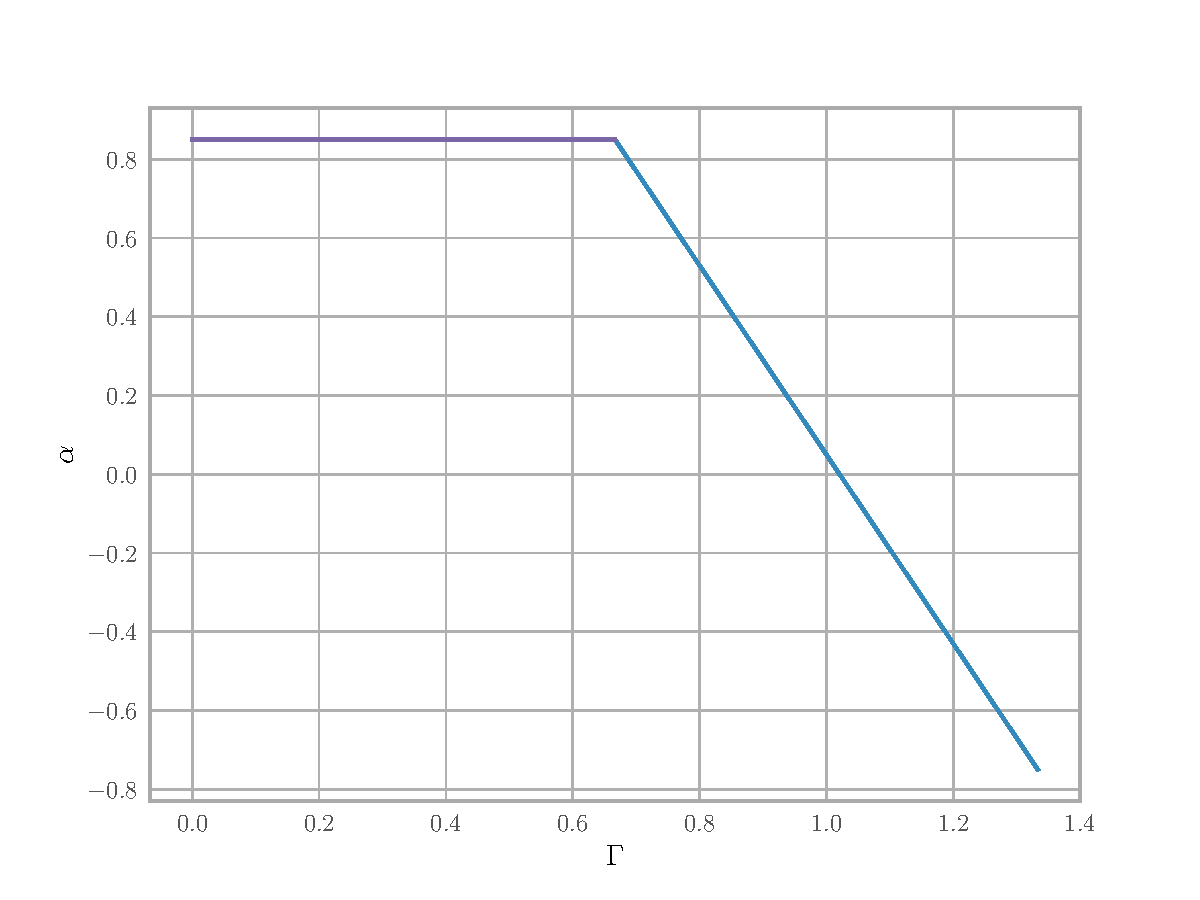
\includegraphics[width=\textwidth]{figures/Eddington_alpha_dependence.pdf}
\caption{}
\label{fig:Eddington_alpha_dependence}
\end{figure}
  
The question is: does the star explode as a CCSN or not? 
If yes, we get a NS or a low-mass BH. 
If no, we have a direct collapse BH: this can be massive!

When the iron core forms, electron degeneracy pressure is the only thing holding up the core. 
When it reaches the Chandrasekhar mass, it collapses, and is then stopped by neutron degeneracy pressure. 

This creates a bounce shock. 
There is a boundary: above it neutrinos fly away, below it the shock is stalled. 

The question is: how is this shock revived? it must be, since we observe CCSNe. 

Maybe there is convection. This should be simulated with 3D simulations, which are very computationally expensive. 

We can get a lower bound on the mass of the envelope: if it is very massive, the star directly collapses. 
The estimate gives \(M > 50 M_{\odot}\). 

The simplest models use the C-O core mass as a parameter. If it is larger than \(8 \divisionsymbol 12 M_{\odot}\) the SN explosion fails. 

Another criterion is the compactness parameter: 
%
\begin{align}
\xi_{M} = \frac{M / M_{\odot}}{R(M) / \SI{1e6}{m}}
\,,
\end{align}
%
which is a multiple of the ratio \(R_{\text{Schwarzschild}} / R\). 

Simulations show that the time for the collapse has an inverse dependence on the compactness parameter. 

There is a correlation between \(\xi \) and \(M_{CO}\). 
However there are researchers who are not convinced that compactness is a good enough estimator. 

The mass of the remnant also depends on the fallback, which is not well understood. 

How fast is the explosion? More importantly: by how much is the revival delayed with respect to the collapse? 

Also, there are also PISNe. These leave no remnant. 
If there is pulsational instability, we have less final mass since more of it is shed. 

Also, we have electron-capture SNe, which form NSs and will be discussed with professor Tauris. 

To wrap up: the main idea is that if there is low metallicity, lower than \(\num{.5} Z_{\odot}\) then stellar winds are quenched, there is larger pre-SN mass, and therefore direct collapse is more likely, so we will have more massive BHs. 

This was first discussed by Heger+ 2003. 
We have plots showing the final mass versus Zero-Age Main Sequence Mass. 
Black line: no mass loss. Blue line: mass of the star at collapse. Red line: mass of the remnant. 
At high metallicity, the mass of the star as collapse is very low.
A zero metallicity, we have two regimes: above a threshold of about \(40 M_{\odot}\) there is direct collapse; below this we have a SN with BH formation. 

What happens for intermediate metallicities? 
It is difficult: we need to account for metals, and we do not have calibration stars in the near universe. 

This depends on the model of stellar winds, but the literature is quite convergent on that. The only big uncertainty is due to rotation and magnetic fields. 

The model also depends on the model of CCSNe, but the main uncertainty is in the low-mass end. This is crucial for our understanding of NS and low-mass BH formation. 

In this area, we cannot be really predictive. 

Are the masses of the detected BHs evidence for population III stars? 
See Hartwig \cite[]{hartwigGravitationalWavesRemnants2016}: it is not very likely. 

\end{document}
